\documentclass{article}
\usepackage[utf8]{inputenc}
\usepackage[T1]{fontenc}
\usepackage{lmodern}
\usepackage{graphicx}
\usepackage{color}
\usepackage{hyperref}
\usepackage{amsmath}
\usepackage{amsfonts}
\usepackage{epstopdf}
\usepackage[table]{xcolor}
% \usepackage{matlab}

\sloppy
\epstopdfsetup{outdir=./}
\graphicspath{ {./ee230_hw1_2442640_2443075_images/} }
% \matlabhastoc

\title{EE 230 Spring 2021-2022 \\ HW 1}
% \author{İsmail Enes Bülbül, Abdullah Emir Göğüsdere}
% \date{March 2022}
\date{}
\author{}

\begin{document}
\maketitle
    \noindent
    \textbf{Group Number: 2443075, 2442630\\
    Group Members: Abdullah Emir Göğüsdere, İsmail Enes Bülbül}
    \section*{1)}
    \subsection*{a)}
    \begin{math}
        \Omega = \{ x | x \in N, x > 0 \} 
    \end{math}
    \\
    The sample space consists of natural numbers greater than 0.
    The number represents number of total flipping before someone wins.
    For example, 2 represents that Ayşe get tail in the first trial,
    and Bora get head in his first trial.
    Any number represents that Ayşe wins if the remainder from the
    division of the number by 3 is 1, and represents Bora wins if
    the remainder is 2, and represents Ceyda wins otherwise.
    \subsection*{b)}
    \begin{math}
        A = \{ x | x \in \Omega, x  \% 3 = 1 \} \\
        B = \{ x | x \in \Omega, x  \% 3 = 2 \} \\
        A\cup B = \{ x | x \in \Omega, x  \% 3 \neq 0 \} \\
        (A\cup B)^c = \{ x | x \in \Omega, x  \% 3 = 0 \} \\
    \end{math}
    \subsection*{c)}
    Let the events \(E_k\) be defined as follows:\\
    \(E_k\): the event for the case that first k-1 trial is tail and kth trial is head.\\
    Then we can write events A and B in terms of \(E_k\) as follows:\\
    \begin{math}
        A = E_1 \cup E_4 \cup E_7 \cup ...\\
        B = E_2 \cup E_5 \cup E_8 \cup ...\\
    \end{math}
    Since these events are disjoint, we can calculate the probabilities as follows:
    \begin{math}
        P(A) = P(E_1) + P(E_4) + P(E_7) + ...\\
        P(B) = P(E_2) + P(E_5) + P(E_8) + ...\\
    \end{math}
    The probability of \(E_k\) can be calculated as:\\
    \begin{math}
        P(E_k) = (1-p)^{k-1}\cdot p\\
    \end{math}
    Then we can calculate \(P(A)\) and \(P(B)\) as:\\
    \begin{math}
        P(A) = \sum_{k=1}^{\infty} (1-p)^{3\cdot(k-1)}\cdot p\\
        = p\cdot(((1-p)^3)^0 + ((1-p)^3)^1 + ((1-p)^3)^2 + ...)
        = \frac{p}{1-(1-p)^3} = \frac{1}{p^2-3p+3}\\\\
        P(B) = \sum_{k=1}^{\infty} (1-p)^{3\cdot(k-1)+1}\cdot p\\
        = p\cdot(1-p)\cdot(((1-p)^3)^0 + ((1-p)^3)^1 + ((1-p)^3)^2 + ...)
        = \frac{p\cdot(1-p)}{1-(1-p)^3} = \frac{1-p}{p^2-3p+3}
    \end{math}
    \subsection*{d)}
    Since events A and B are disjoint, by axiom 2, we have \\
    \begin{math}
        P(A\cup B) = P(A) + P(B) = \frac{1}{p^2-3p+3}
        +\frac{1-p}{p^2-3p+3}
        =\frac{2-p}{p^2-3p+3} \\\\
    \end{math}
    Since \((A\cup B)\) and\((A\cup B)^c\) are disjoint, 
    and \(\Omega = (A\cup B) + (A\cup B)^c\) we have \\
    \begin{math}
        P((A\cup B)^c) = P(\Omega) - P(A\cup B)\\
    \end{math}
    By axiom 3, \(P(\Omega) = 1\). Therefore \(P((A\cup B)^c) = \frac{p^2-2p+1}{p^2-3p+3}\)
    \subsection*{e)}
    For A and B: \\
    \(P(A) + P(B) - 1 = \frac{2-p}{p^2-3p+3} - 1
    = \frac{-p^2+2p-1}{p^2-3p+3} = \frac{-(p-1)^2}{(p-3/2)^2+3/4} \leq 0 \,\, \forall p \,\, 0 \leq p \leq 1\)\\
    \(P(A\cap B) = 0\) (events are disjoint)\\
    \(0 \geq \frac{-(p-1)^2}{(p-3/2)^2+3/4}\) (equation holds)    \\\\
    For arbitrary two events C and D: \\
    \begin{math}
        P(C\cap D) \geq P(C) + P(D) -1\\
        P(C\cap D) \geq P(C \backslash  D) + P(D \backslash  C) + 2P(C\cap D) - 1\\
        1 \geq P(C \backslash  D) + P(D \backslash  C) + P(C\cap D)\\
        1 \geq P(C\cup D)
    \end{math}
     (equation holds)

    \section*{2)}
    \subsection*{a)}
    \begin{math}
        B: A_3 \cap A_5 \,\, given \,\, A_2
    \end{math}
    \subsection*{b)}
    \begin{math}
        P(B) = P(A_3 \cup A_5 | A_2) = \frac{P(A_2 \cap (A_3 \cup A_5))}{P(A_2)}
        = \frac{P((A_2 \cap A_3)\cup(A_2 \cap A_5))}{P(A_2)}\\
        = \frac{P((A_2 \cap A_3)) + P((A_2 \cap A_5)) - P((A_2 \cap A_3 \cap A_5))}{P(A_2)}\\
    \end{math}
         \(A_2 = \{ 2, 4, 6, ..., 100 \}\) has 50 elements\\
         \(A_2 \cap A_3 = \{ 6, 12, 18, ..., 96 \}\) has 16 elements\\ 
         \(A_2 \cap A_5 = \{ 10, 20, 30, ..., 100 \}\) has 10 elements\\ 
         \(A_2 \cap A_3 \cap A_5 = \{ 30, 60, 90 \}\) has 3 elements\\
    \begin{math}
        \frac{P((A_2 \cap A_3)) + P((A_2 \cap A_5)) - P((A_2 \cap A_3 \cap A_5))}{P(A_2)} = \frac{0.16 + 0.1 - 0.03}{0.5} = 0.58
    \end{math}
    \subsection*{c)}
    \begin{math}
        P(A_a \cup A_b | A_2) = \frac{A_2\cap (A_a \cup A_b)}{P(A_2)}
        = \frac{P(A_2 \cap A_a) + P(A_2 \cap A_b) - P(A_2 \cap A_a \cap A_b)}{P(A_2)}\\
    \end{math}
    If we assume that \(a\neq b\), \(a\neq 2\), and \(b\neq 2\); than we have\\
    \begin{math}
        P(A_a \cup A_b | A_2)= \frac{P(A_{2a}) + P(A_{2b}) - P(A_{2ab})}{P(A_2)}\\
    \end{math}
    To obtain a formula for general case (without any assumption like \(a\neq 2\))
    we can divide subscripts in the numerator by the greatest common dividor.
    Therefore our formula will be \\
    \begin{math}
        P(A_a \cup A_b | A_2)=
        \frac{ P(A_{\frac{2a}{\gcd(2,a)}}) + P(A_{\frac{2b}{\gcd(2,b)}}) - P(A_{\frac{2ab}{\gcd(2,a) \cdot \gcd(a,b)}})}{P(A_2)}\\
    \end{math}
    \section*{3)}
    Let the events \(A_k\) and \(B\) be defined as :\\
    \(A_k\): The event that the family has k children\\
    \(B\): The event that the chosen child is the youngest one\\
    \(B'\): The event that the chosen child is the oldest one\\
    By theorem 2: \\
    \begin{math}
        P(B|A_k) = P(B'|A_k) = 1/k\\
        P(B') = \sum_{k=1}^{4} P(B'|A_k)\cdot P(A_k) = \sum_{k=1}^{4} (1/k)\cdot p_k\\
        P(B) = \sum_{k=1}^{4} P(B|A_k)\cdot P(A_k) = \sum_{k=1}^{4} (1/k)\cdot p_k\\
        P(B) = P(B') = 0.25 + 0.45/2 + 0.2/3 + 0.1/4 = 0.56\\
        P(A_k|B) = \frac{P(B|A_k)\cdot P(A_k)}{P(B)} = \frac{(1/k)\cdot p_k}{0.56}
    \end{math}
    \subsection*{a)}
    \begin{math}
        P(A_1|B) = \frac{p_k}{0.56k} = 0.25/0.56 = 0.45
    \end{math}
    \subsection*{b)}
    \begin{math}
        P(A_3|B) = \frac{p_k}{0.56k} = 0.2/(3*0.56) = 0.12
    \end{math}
    \subsection*{c)}
    \(P(B') = 0.56\)
    \section*{4)}
    \subsection*{a)}
    \begin{math}
        {5 \choose 3} \cdot p^3 \cdot q^2 = 10\cdot p^3 \cdot q^2  
    \end{math}
    \subsection*{b)}
    Let the index of the first outcome \(\omega _q\) be n, 
    then we should have outcomes \(\omega _p\) or \(\omega _r\)
    for the indexes between 1 and n-1. We can calculate this probability as:\\
    \begin{math}
        \sum_{k=2}^{5} (1-q)^{n-1}\cdot q\\
    \end{math}
    But we have to remove the case that all outcomes before nth trial is \(\omega _r\), 
    so our formula will be:\\
    \begin{math}
        \sum_{k=2}^{5} ((1-q)^{n-1} - r^{n-1})\cdot q =
        q\cdot \sum_{k=1}^{4} ((1-q)^n - r^n)
    \end{math}
    \subsection*{c)}
    We can use the formula with replacing the upper limit
    of summation with \({\infty}\).\\
    \begin{math}
        q\cdot \sum_{k=1}^{\infty} ((1-q)^n - r^n) = q\cdot (\frac{1}{1-(1-q)} - \frac{1}{1-r})
        = 1 - \frac{q}{1-r} = \frac{1 - r - q}{1 - r} = \frac{p}{1 - r}
    \end{math}
    

    % % This LaTeX was auto-generated from MATLAB code.
    % % To make changes, update the MATLAB code and export to LaTeX again.
    % \section*{5)}
    % \label{T_132C85D7}
    % \matlabtitle{EE230 HW1 MATLAB Question: Parameter Estimation}

    % \begin{par}
    % \begin{center}
    % \textit{İsmail Enes Bülbül, Abdullah Emir Göğüsdere}
    % \end{center}
    % \end{par}

    % \begin{par}
    % \begin{center}
    % \textit{2442630, 2443075}
    % \end{center}
    % \end{par}

    % \matlabtableofcontents{Table of Contents}
    % \label{H_440FC271}
    % \matlabheading{Task: Estimating the probability of success from Bernoulli trials.}

    % \begin{par}
    % \begin{flushleft}
    % The Bernoulli random variable is a mathematical abstraction for a possibly unfair coin toss, expressed as follows:
    % \end{flushleft}
    % \end{par}

    % \begin{par}
    % $$X\in \lbrace 0,1\rbrace ~~~~\textrm{P}(X=1)=p,\,\,\,\textrm{P}(X=0)=1-p,\,\,\,p\in [0,1]$$
    % \end{par}

    % \begin{par}
    % \begin{flushleft}
    % The $X=1$ case is called a \textit{success}, and consequently $X=0$ is called as \textit{failure}. In this work, you will be trying to estimate the probability of success $p$ of a Bernoulli random variable from \texttt{N} independent \& identically distributed (iid.) samples. 
    % \end{flushleft}
    % \end{par}


    % \label{H_A0F6F3AC}
    % \matlabheadingtwo{Part I. Sampling}

    % \begin{par}
    % \begin{flushleft}
    % You will begin by using \texttt{randsample()} to take independent identically distributed (iid.) samples from the random variable described above. Think about discrete probabilistic model given above: What is the sample space, elementary events, and the assigned probabilities to these elementary events? How do they correspond to the arguments of \texttt{randsample()}?
    % \end{flushleft}
    % \end{par}

    % \begin{itemize}
    % \setlength{\itemsep}{-1ex}
    % \item{\begin{flushleft} Assign a variable \texttt{N} for the number of samples, and adjust its value with a numeric slider that ranges from \texttt{10} to \texttt{1000} in steps of \texttt{10}. Have the control run the current section as its value is changing. \end{flushleft}}
    % \item{\begin{flushleft} Assign a variable \texttt{p} for the probability of success, and use a numeric slider to adjust its value.  Have the control run the current section as its value is changing. \end{flushleft}}
    % \item{\begin{flushleft} Use the function \texttt{randsample()} to generate \texttt{N} samples with probability of success \texttt{p}. Consult \texttt{help randsample} to figure out how the function works, if you need to.  \end{flushleft}}
    % \end{itemize}

    % \begin{matlabcode}
    % clear variables; close all; clc;
    % N = 1000;
    % p = 0.7;

    % samples = randsample([0 1],N,true,[1-p p]);
    % \end{matlabcode}

    % \begin{par}
    % \begin{flushleft}
    % Now for some visualization.
    % \end{flushleft}
    % \end{par}

    % \begin{itemize}
    % \setlength{\itemsep}{-1ex}
    % \item{\begin{flushleft} Use \texttt{histogram()} to plot how many of which outcome has been sampled. Prettify the plot. \end{flushleft}}
    % \end{itemize}

    % \begin{matlabcode}
    % figure

    % histogram(samples)
    % \end{matlabcode}
    % \begin{center}
    % 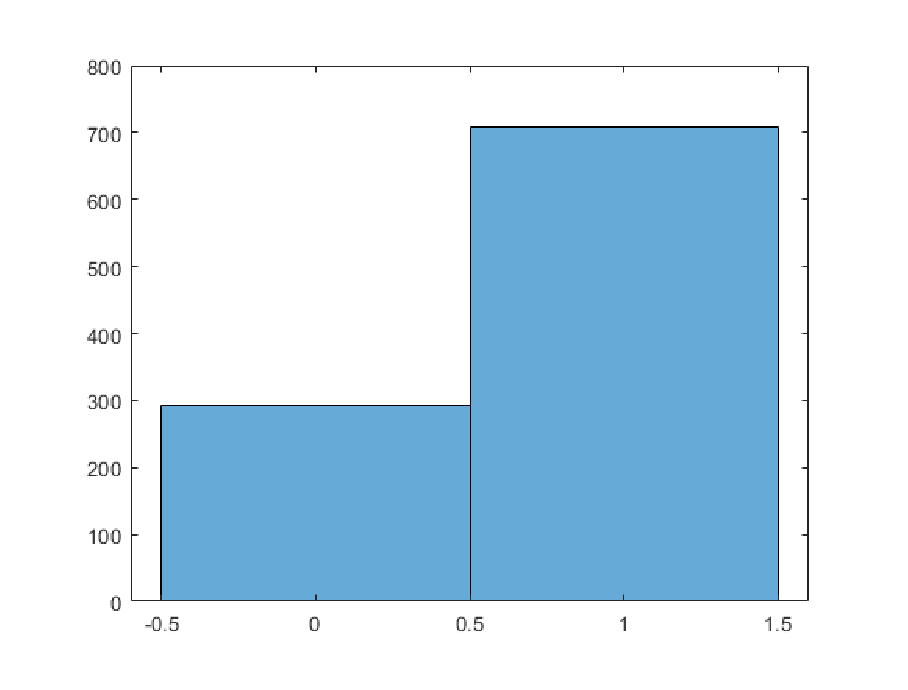
\includegraphics[width=\maxwidth{56.196688409433015em}]{figure_0.eps}
    % \end{center}


    % \label{H_25EBD824}
    % \matlabheadingtwo{Part II. Estimation}

    % \begin{par}
    % \begin{flushleft}
    % Now that you have your samples, let's do some parameter estimation. You will try to estimate the probability of success via the most intuitive formula: Number of successes divided by the total number of trials.
    % \end{flushleft}
    % \end{par}

    % \begin{itemize}
    % \setlength{\itemsep}{-1ex}
    % \item{\begin{flushleft} Use the previously generated samples and apply this formula to estimate the probability of success. \end{flushleft}}
    % \end{itemize}

    % \begin{matlabcode}
    % p_est = sum(samples(:) == 1)/N
    % \end{matlabcode}
    % \begin{matlaboutput}
    % p_est = 0.6910
    % \end{matlaboutput}

    % \begin{par}
    % \begin{flushleft}
    % What you code above is called an \textit{estimator}: A function that maps the observed samples to the estimate of the quantitiy in question. You will want to convert your estimator to a stand-alone MATLAB function, so that it may be called when needed.
    % \end{flushleft}
    % \end{par}

    % \begin{itemize}
    % \setlength{\itemsep}{-1ex}
    % \item{\begin{flushleft} Complete the empty function \texttt{estimator()} in \hyperref[H_9C34D6E2]{Appendix A.1.} and call it once more below to make sure it works. \end{flushleft}}
    % \end{itemize}

    % \begin{matlabcode}
    % p_est = estimator(samples)
    % \end{matlabcode}
    % \begin{matlaboutput}
    % p_est = 0.6910
    % \end{matlaboutput}


    % \label{H_4671C279}
    % \matlabheadingtwo{Part III. Evaluation}

    % \begin{par}
    % \begin{flushleft}
    % In this final part, you are asked to evaluate the success of your estimator as a function of number of observations. 
    % \end{flushleft}
    % \end{par}

    % \begin{itemize}
    % \setlength{\itemsep}{-1ex}
    % \item{\begin{flushleft} Generate a new, "big" data set of \texttt{N = 1000} samples, again with \texttt{p} adjusted with a numeric slider. \end{flushleft}}
    % \item{\begin{flushleft} Write a \texttt{for} loop to use your estimator with the first \texttt{n} samples \textit{of the dataset you generate in this section} where \texttt{n} varies from \texttt{1} to \texttt{N}, and record the estimator output to a vector. \end{flushleft}}
    % \item{\begin{flushleft} Plot the estimator output as a function of the number of observed samples. On the same plot, plot a horizontal line that is equal to the value of true \texttt{p}, so that it is easier to compare the estimated value to the true one. \end{flushleft}}
    % \item{\begin{flushleft} Have the final estimate of \texttt{p} and the true \texttt{p} printed in the title of the plot. This title must adapt to the final estimate and \texttt{p} value as set by the numeric slider.  \end{flushleft}}
    % \item{\begin{flushleft} Add a button control to rerun this section for a new data set of same size, and observe whether different estimated p vs. nr. of samples used converge to the same final \texttt{p} estimate. \textbf{Bonus:} Plot different realizations of these plot \textit{on the same figure }multiple (5-10 should be plenty). If you do so, you can choose either run's final estimate to show in the title. \end{flushleft}}
    % \end{itemize}

    % \begin{matlabcode}
    % f = figure;
    % f.Position = [0 0 1000 600];

    % p = 0.7;
    % N = 1000;
    % data = randsample([0 1],N,true,[1-p p]);

    % p_est_ = ones(1,N);

    % for n = 1:N
        
    %     p_est_(n) = estimator(data(1,1:n));

    % end

    % plot(p_est_)
    % hold on;
    % plot(p*ones(1,N))

    % xlim([0 1000])
    % ylim([0 1.1])
    % legend("pEstimated", "p")
    % title("Estimated p = " +  p_est_(1,N) + ", True p = " + p)
    % ylabel("Probability")
    % xlabel("Samples")
    % \end{matlabcode}
    % \begin{center}
    % 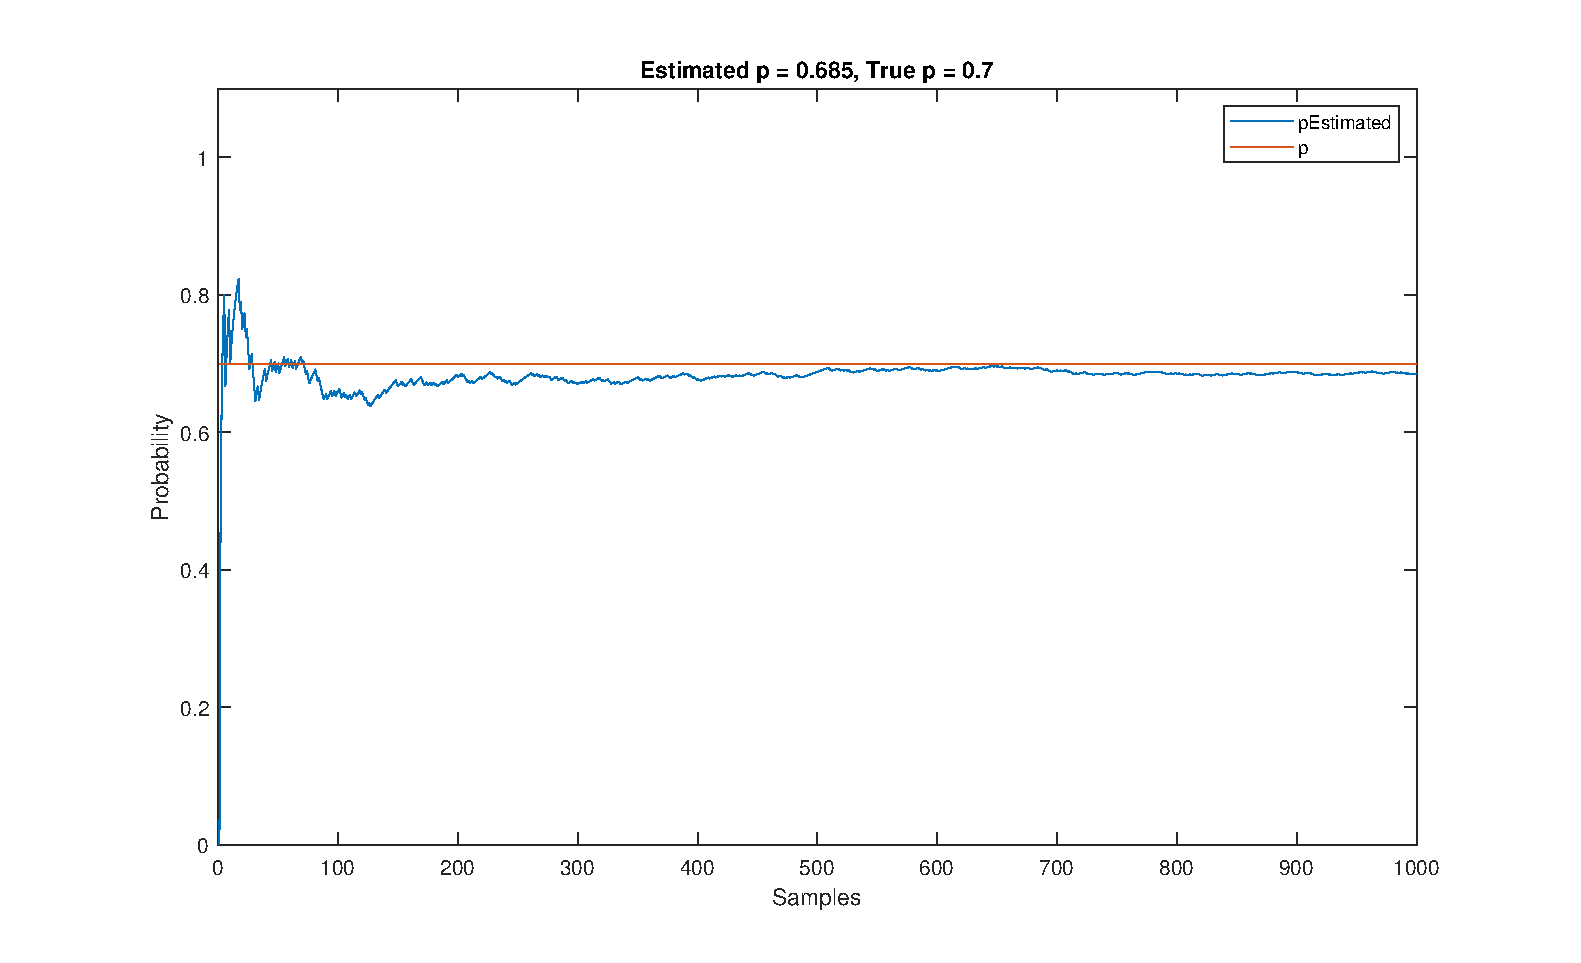
\includegraphics[width=\maxwidth{100.35122930255896em}]{figure_1.eps}
    % \end{center}
    % \begin{matlabcode}
    
    % \end{matlabcode}


    % \begin{par}
    % \begin{flushleft}
    % \textbf{Bonus:}
    % \end{flushleft}
    % \end{par}

    % \begin{matlabcode}
    % hold off; close all;
    % f = figure;
    % f.Position = [0 0 1000 600];

    % numExp = 5;
    % pEst = string(zeros(1,numExp));

    % for repeat = 1:numExp
    %     data = randsample([0 1],N,true,[1-p p]);
        
    %     p_est_ = ones(1,N);
        
    %     for n = 1:N
            
    %         p_est_(n) = estimator(data(1,1:n));
        
    %     end
    %     pEst(1,repeat) = "Exp" + ...
    %     string(repeat) + ": " + string(p_est_(1,N));

    % plot(p_est_)
    % hold on;

    % end

    % pEst = [string(pEst), "True: " + string(p)];

    % plot(p*ones(1,N))
    % title(join(pEst,", "))
    % legend(pEst)
    % ylabel("Probability")
    % xlabel("Samples")
    % hold off;
    % \end{matlabcode}
    % \begin{center}
    % 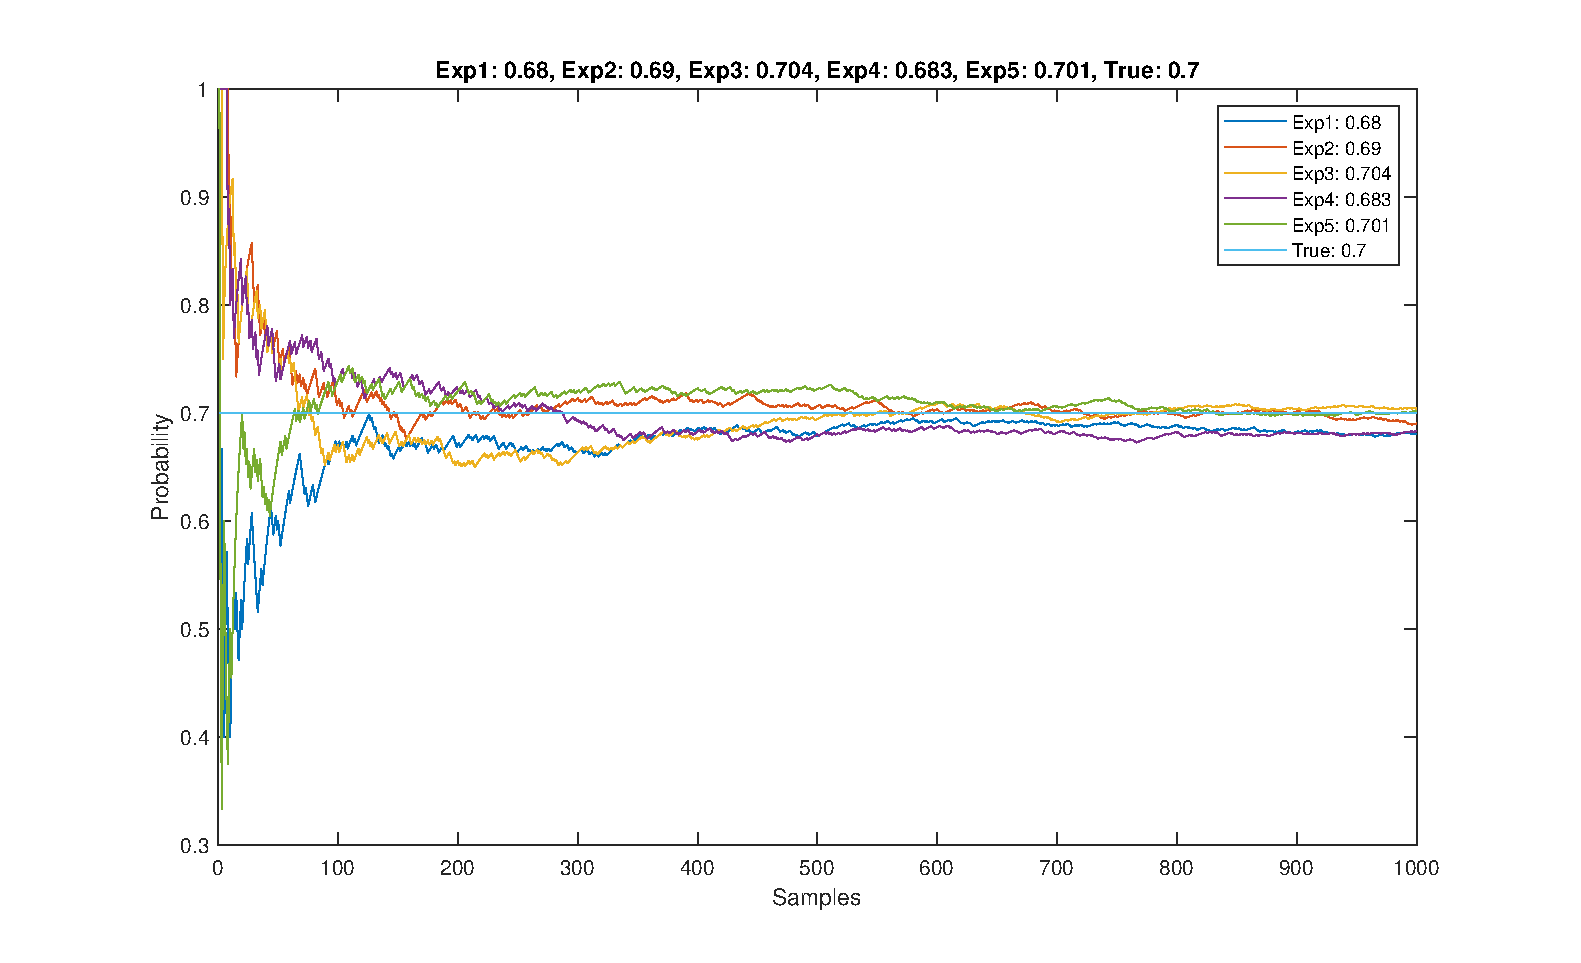
\includegraphics[width=\maxwidth{100.35122930255896em}]{figure_2.eps}
    % \end{center}


    % \begin{itemize}
    % \setlength{\itemsep}{-1ex}
    % \item{\begin{flushleft} Comment briefly on the behaviour you observe on the plot you create above. How does your estimator perform? Do the plots vary from run to run? What are the similarities and differences between different runs? \end{flushleft}}
    % \end{itemize}

    % \begin{par}
    % \begin{flushleft}
    % From the above plots, as we increase the portion of the \textbf{data} to be calculated in each loop until it reaches the whole portion, it can be seen that the \textbf{pEstimated} converges to the true \textbf{p}. Therefore, we can say that the \textbf{estimator} performs sufficiently. Moreover, we can see that the plots vary from run to run since the \textbf{randsample()} creates \textbf{N}-sized samples randomly and closely weighted to true \textbf{p}. 
    % \end{flushleft}
    % \end{par}

    % \begin{par}
    % \begin{flushleft}
    % The difference between runs is that the \textbf{data} sets in each run are created randomly and closely weighted to true p, so the data sets in each run are not the same. Although this is the case, their similarity is that their \textbf{pEstimated} will eventually converge to the true \textbf{p}.
    % \end{flushleft}
    % \end{par}

    % \label{H_96AE8304}
    % \matlabheading{Appendix A. Function Declarations}

    % \label{H_9C34D6E2}
    % \matlabheadingtwo{A.1. Your Estimator}

    % \begin{matlabcode}
    % function [p_est] = estimator(samples)
    %     [p_est] = sum(samples(:) == 1)/length(samples);
    % end
    % \end{matlabcode}

\end{document}
